\subsection{Eksempel: FIFA-skillz}
Spillet FIFA 20 gir poengscorer til ferdighetene til et lass med fotballspillere. For utespillere er det 34 ulike ferdigheter som rangeres på en skala fra 1 til 99. Fra disse regnes det ut seks nøkkelscorer: Sprinthastighet, Skudd, Pasninger, Dribling, Forsvarsspill og Fysikk. Til slutt tildeles hver spiller en overall-score, som \textit{Ikke regnes ut direkte fra ferdighetene som bestemmer hvordan spilleren oppfører seg i spillet}. I tillegg til en vektet sum av disse ferdighetene (vektingen er avhengig av spillerens posisjon) legges til til en ``Internasjonalt rykte''-score, som betyr at spillernes endelige score er mer en subjektiv vurdering av hvor ``god'' den ekte spilleren er, enn en vurdering av hvilke spillere det lønner seg å bruke når man spiller FIFA.

Til å begynne med kan vi dermed konkludere med at man ikke burde se på overall-score for å vurdere hvilke spillere man burde bruke når man spiller, men heller se på sekskanten med nøkkelferdigheter som dukker opp for hver spiller.

Dette betyr imidlertid ikke at overall-score er feil, den er bestemt av veldig kompentente folk som ville gjort bedre spillerkjøp enn en enkel student utstyrt med en datamaskin og et datasett. Jeg antar derfor at overall-scoren som er angitt på FIFA er fasiten på hvor god en spiller er. Om vi ikke har tilgang til denne fasiten, hvor godt kan vi forutse hvor god en spiller er på ekte basert på hvor god spilleren er på FIFA?

La osss begynne å se på hva slags data vi har å jobbe med. Figur \ref{fig:fifa-pca1} viser oversiktsplott for PCA utført på 400 tilfeldig valgte fotballspillere sine ferdigheter. Denne dataen utgjør vår $X$. Denne dataen inkluderer ikke nøkkelferdigheter og overall-score, som er utledet med utgangspunkt i $X$ og vil være vår $Y$ i senere analyse. Fra score-plottet kan vi se at keeperne tydelig kommer fra en annen populasjon enn utespillere. Selv om vi ser at modellen klarer å plukke opp mye av variansen i dataen likevel definerer jeg et nytt testsett uten keepere, som anatgeligvis heller burde analyseres hver for seg siden det er så stor forskjell på hvilke ferdigheter som sees på som viktige. 


\begin{figure}[h]
 	\centering
 	\begin{subfigure}[t]{0.48\textwidth}
 		\centering
 		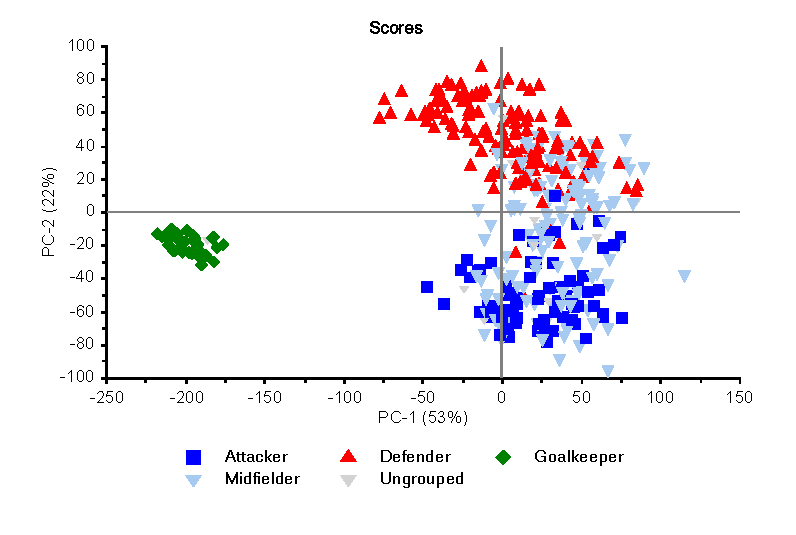
\includegraphics[width=\textwidth]{figurer/fifa-pca1-scores}
 		\caption{}
 		\label{}
 	\end{subfigure}	
 	\begin{subfigure}[t]{0.48\textwidth}
 		\centering
 		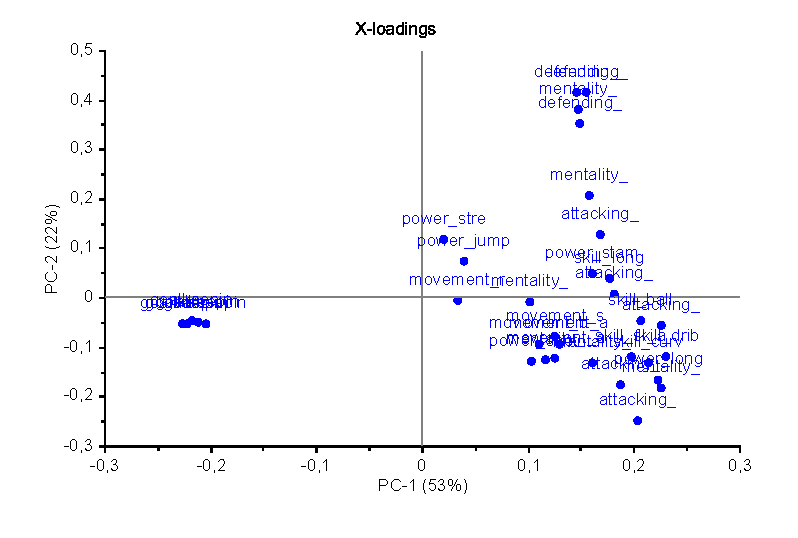
\includegraphics[width=\textwidth]{figurer/fifa-pca1-loadings}
 		\caption{}
 		\label{}
 	\end{subfigure}
 	\begin{subfigure}[t]{0.48\textwidth}
 		\centering
 		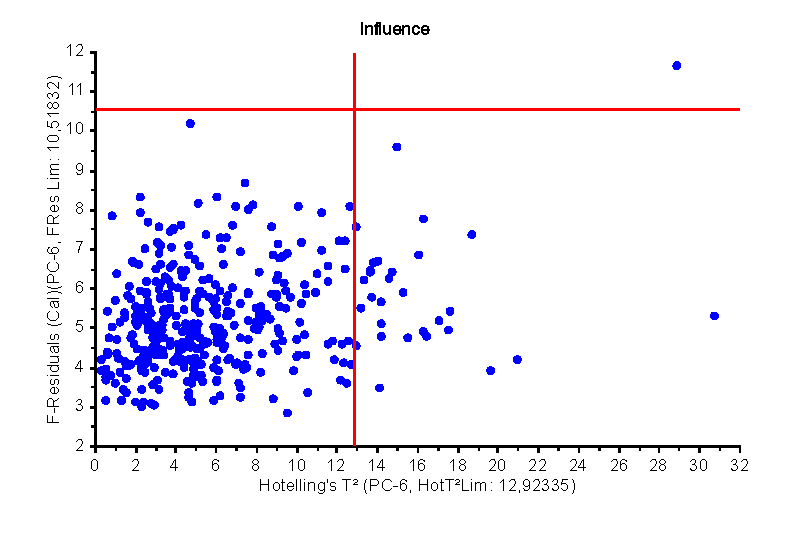
\includegraphics[width=\textwidth]{figurer/fifa-pca1-influence}
 		\caption{}
 		\label{}
 	\end{subfigure}
 	\begin{subfigure}[t]{0.48\textwidth}
 		\centering
 		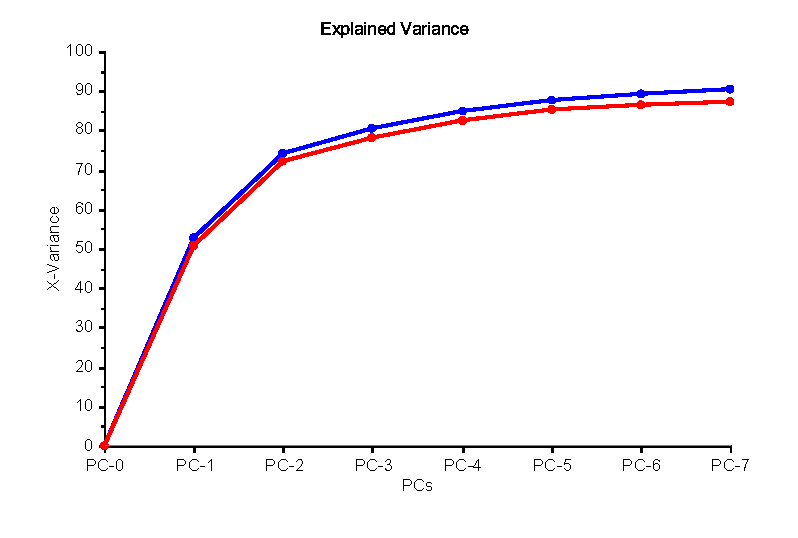
\includegraphics[width=\textwidth]{figurer/fifa-pca1-ev}
 		\caption{}
 		\label{}
 	\end{subfigure}
	\label{fig:fifa-pca1}
	\caption{PCA av fotballspillerferdigheter}
 \end{figure}

 I figur \ref{fig:fifa-pca2} er keeperne utelatt. Vi ser at modellen fortsatt skiller mellom spillernes posisjon, og at dette skjer både langs $PC_1$ og $PC_2$. Midtbanespillere befinner seg i begge klyngene av både forsvars- og angrepsspillere, som ikke er spesielt overraskende. Score-plottet viser at den faktiske posisjonen spillere har på klubblaget sitt ikke nødvendigvis er et godt mål på om de har \textbf{Offensive fibre\texttrademark} eller \textbf{Defensive fibre\texttrademark} i kroppen sin. Loading-plottet viser at de aller fleste ferdighetene bidrar til å forklare en merkbar andel av dataen, med unntak av keeperferdigheter. Vi ser imidlertid at tekniske ferdigheter har større påvirkning enn fysiske, som trolig er jevnere fordelt over alle spillere, uavhengig av posisjon. Influence-plottet viser én ekstrem utligger, som viser seg å være en keeper som har sluppet unna filtreringen.

\begin{figure}[h]
 	\centering
 	\begin{subfigure}[t]{0.48\textwidth}
 		\centering
 		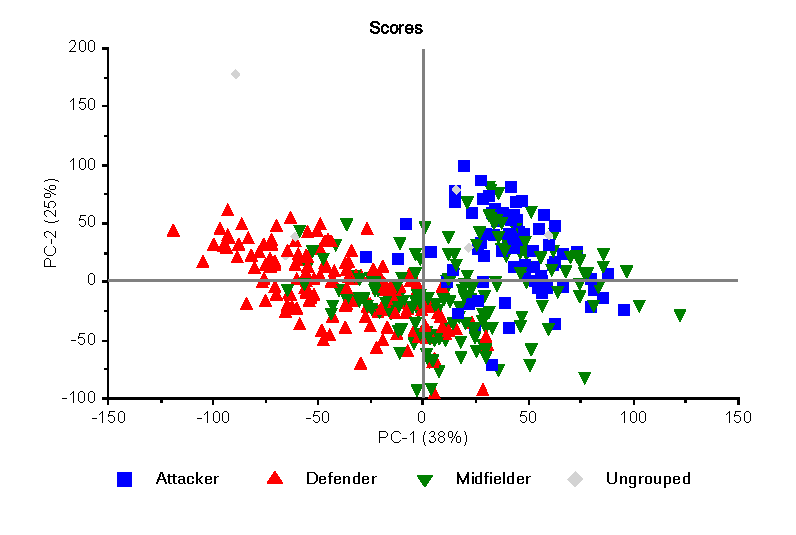
\includegraphics[width=\textwidth]{figurer/fifa-pca2-scores}
 		\caption{}
 		\label{}
 	\end{subfigure}	
 	\begin{subfigure}[t]{0.48\textwidth}
 		\centering
 		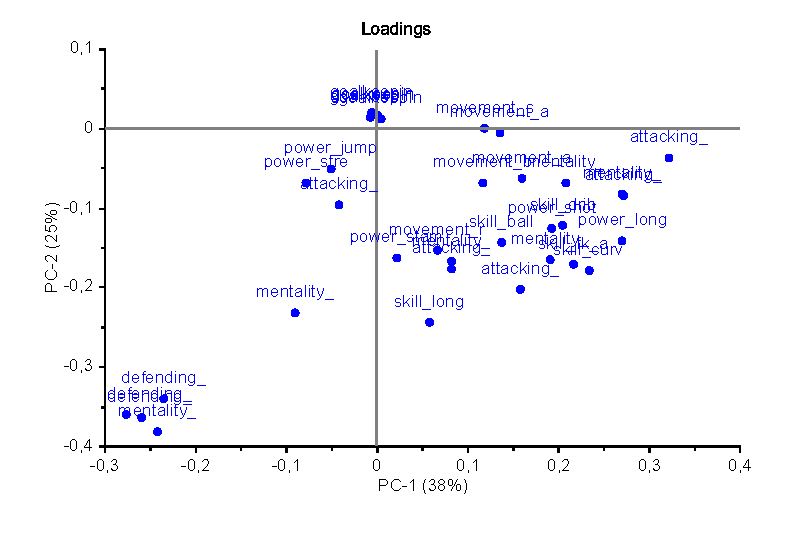
\includegraphics[width=\textwidth]{figurer/fifa-pca2-loadings}
 		\caption{}
 		\label{}
 	\end{subfigure}
 	\begin{subfigure}[t]{0.48\textwidth}
 		\centering
 		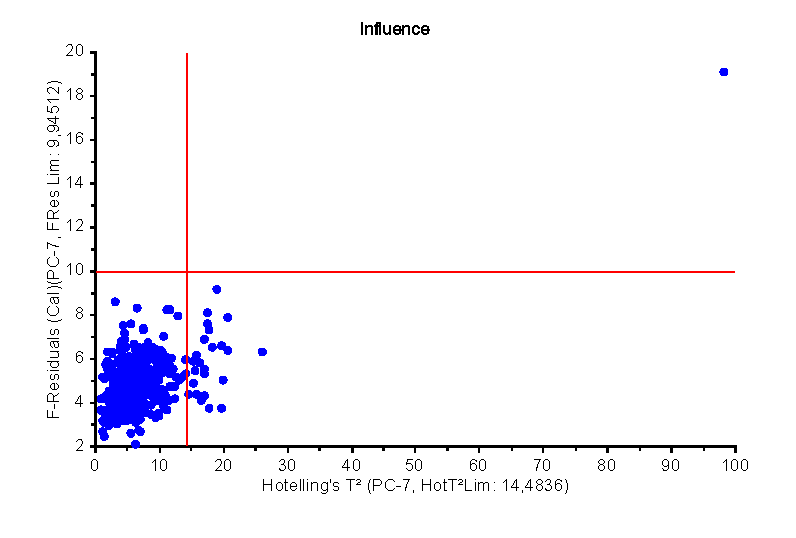
\includegraphics[width=\textwidth]{figurer/fifa-pca2-influence}
 		\caption{}
 		\label{}
 	\end{subfigure}
 	\begin{subfigure}[t]{0.48\textwidth}
 		\centering
 		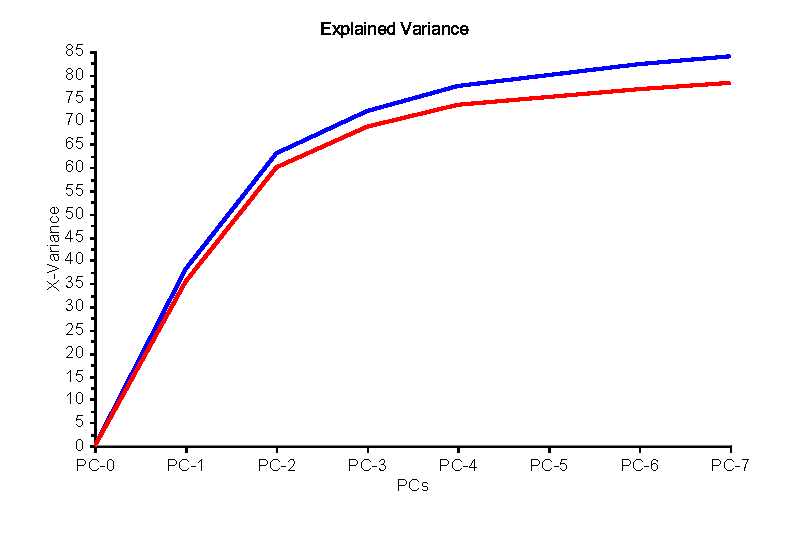
\includegraphics[width=\textwidth]{figurer/fifa-pca2-ev}
 		\caption{}
 		\label{}
 	\end{subfigure}
	\label{fig:fifa-pca2}
	\caption{PCA av fotballspillerferdigheter, uten keeepere}
 \end{figure}

 Figur \ref{fig:fifa-pls} viser PLS-regresjon fra ferdigheter $X$ til overall-score $Y$. Faktorene som forklarer hvilke ferdigheter som henger sammen med høy overall-score skiller fortsatt på posisjon på banen, men denne gangen først og frems langs faktor nr. 2. Den første faktoren henger først og fremst sammen med tekniske ferdigheter, mens andre faktor som nevnt henger sammen med hvor god spilleren er i forsvar/angrep. Loading-plottet forteller oss noe viktig: Fysikk henger lite sammen med overall-score. Dette kan tyde på at ferdigheter som er lette å kvantifisere og implementere i et spill (som f.eks. sprinthastighet og styrke) har mer å si på FIFA enn de har på ekte. Ferdigheter som spilleforståelse kan ikke implementeres på samme måte (de må den som spiller stå for), og dermed vil man aldri ha samme fordel av å f.eks. ha Allan Gaarde på laget sitt på FIFA som man ville hatt i den virkelige verden. EV-plottet viser at omtrent 80\% av variansen i $Y$ kan forklares fra variasjon i $X$, som gir en ganske lav grense for hva vi kan forvente av ytelse for prediksjon av overall-score basert på FIFA-skillz.

\begin{figure}[h]
 	\centering
 	\begin{subfigure}[t]{0.48\textwidth}
 		\centering
 		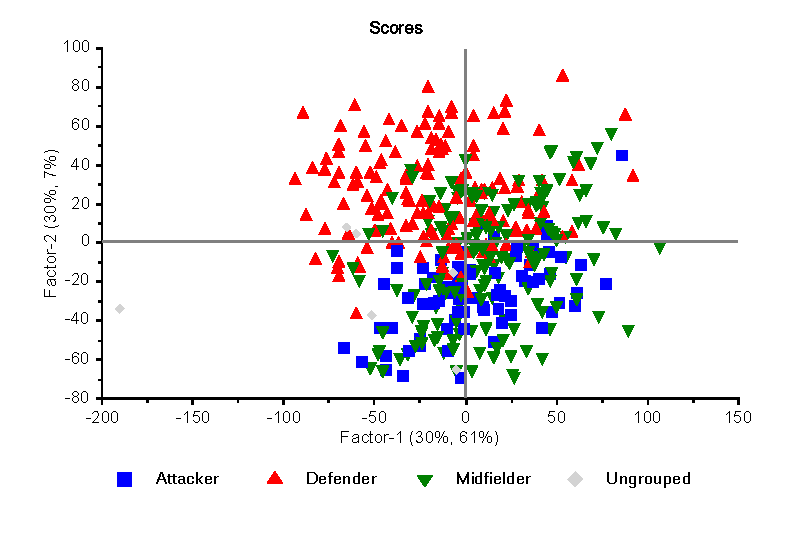
\includegraphics[width=\textwidth]{figurer/fifa-pls-scores}
 		\caption{}
 		\label{}
 	\end{subfigure}	
 	\begin{subfigure}[t]{0.48\textwidth}
 		\centering
 		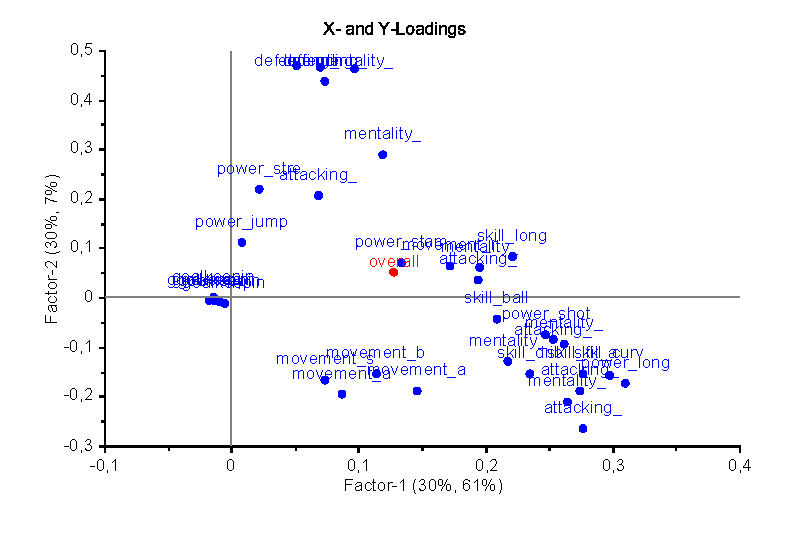
\includegraphics[width=\textwidth]{figurer/fifa-pls-loadings}
 		\caption{}
 		\label{}
 	\end{subfigure}
 	\begin{subfigure}[t]{0.48\textwidth}
 		\centering
 		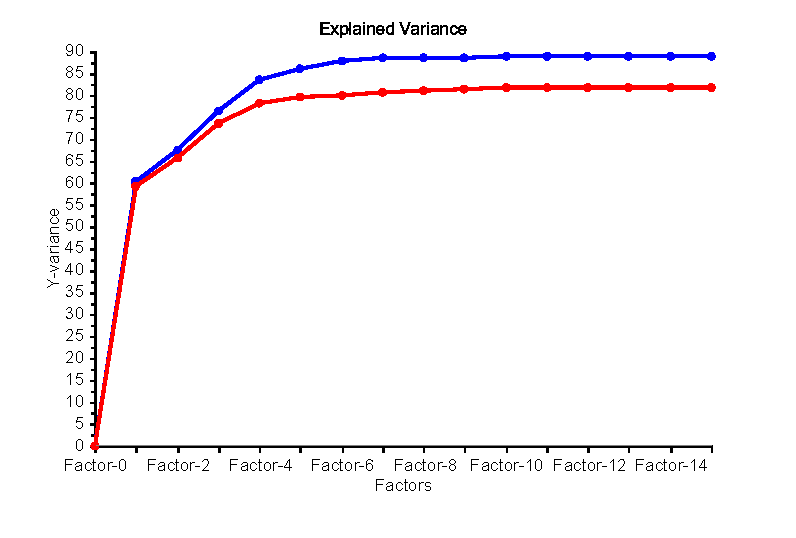
\includegraphics[width=\textwidth]{figurer/fifa-pls-ev}
 		\caption{}
 		\label{}
 	\end{subfigure}
 	\begin{subfigure}[t]{0.48\textwidth}
 		\centering
 		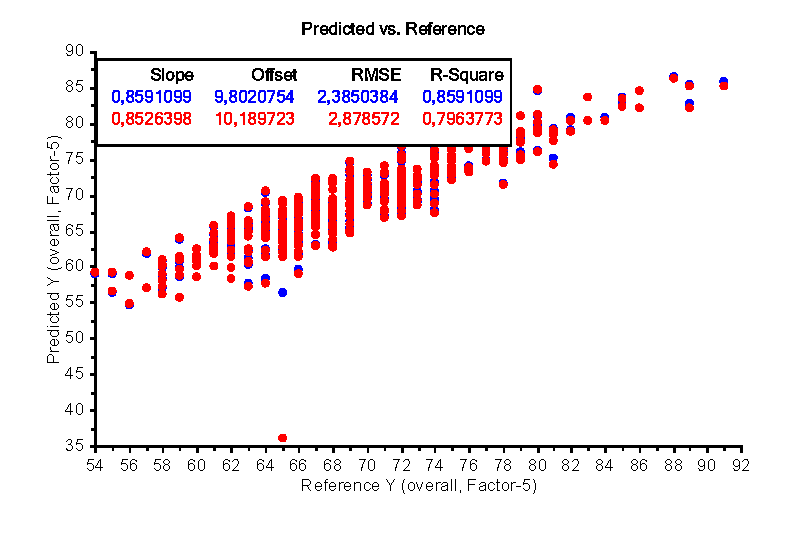
\includegraphics[width=\textwidth]{figurer/fifa-pls-pvsr}
 		\caption{}
 		\label{}
 	\end{subfigure}
	\label{fig:fifa-pls}
	\caption{PLS av fotballspillerferdigheter, uten keeepere}
 \end{figure}

 La oss prøve likevel. Figur \ref{fig:fifa-pls-train-vs-test} viser resultatet av å bruke PLS-modellen diskutert over til å predikere overall-score basert på FIFA-ferdigheter på hhv. treningssettet med 400 spillere og testsettet med 200 spillere. Testsettet har en $R^2$ på $0,82$, som er noe lavere enn $0,86$, som er verdien for treningssettet. Begge disse er imidlertid ganske tett opp mot grensen for variansen i $Y$ som kan forklares som en lineær funksjon av $X$. Regresjonslinjene for begge figurer viser tydelig problemet med å tilpasse en lineær modell: Spillere som er gode på FIFA (høye verdier i $X$) er typisk så gode på ekte at overall-score ($Y$) justeres opp.

\begin{figure}[h]
	\centering
	\begin{subfigure}[t]{0.96\textwidth}
		\centering
		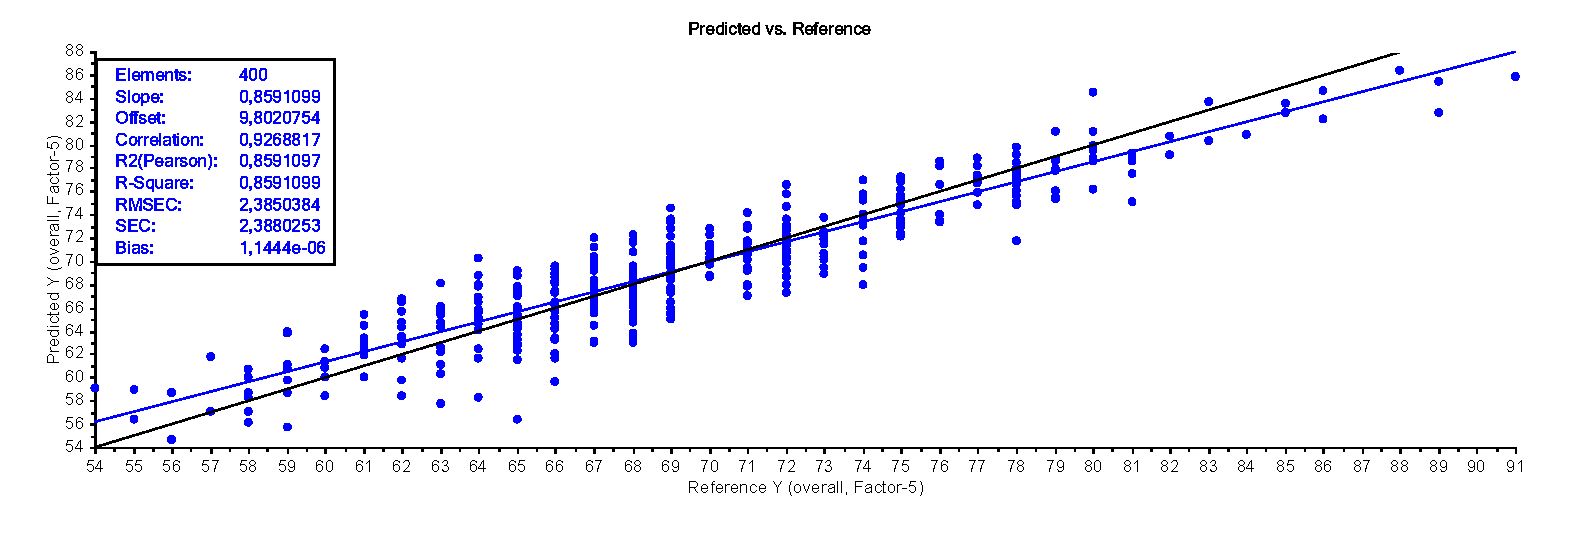
\includegraphics[width=\textwidth]{figurer/fifa-pls-training-pvsr}
		\caption{Treningssett}
		\label{}
	\end{subfigure}
	\begin{subfigure}[t]{0.96\textwidth}
		\centering
		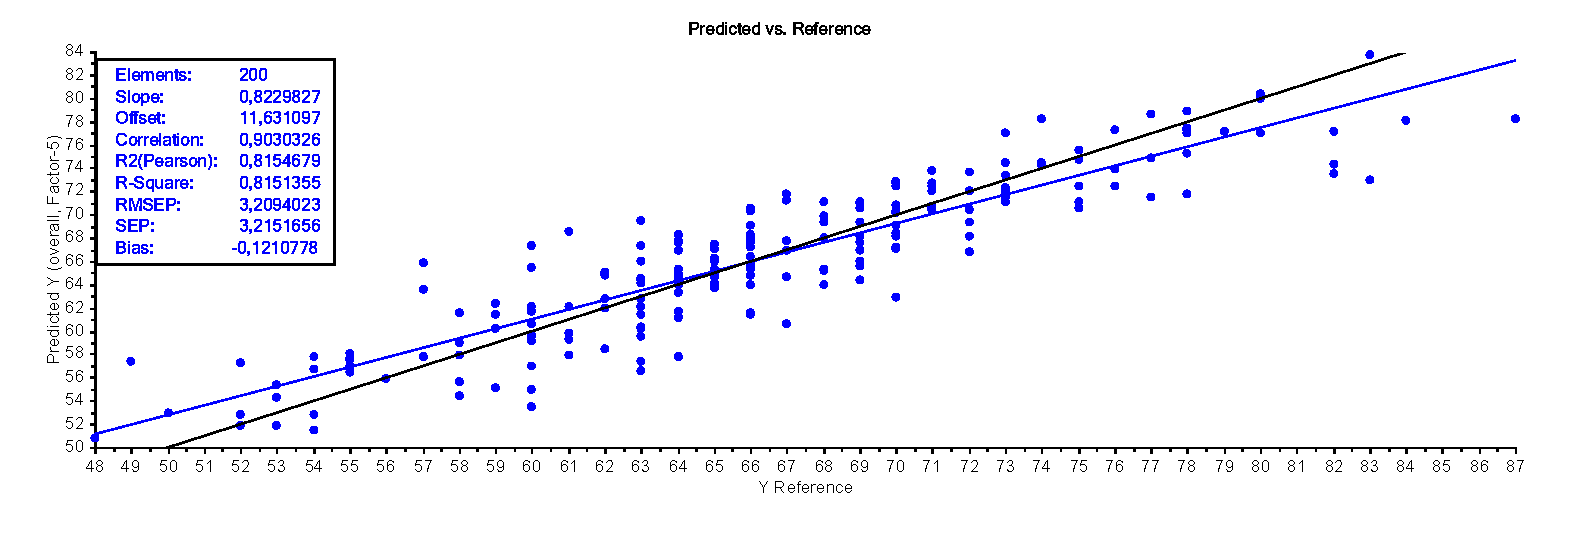
\includegraphics[width=\textwidth]{figurer/fifa-pls-test-pvsr}
		\caption{Testsett}
		\label{}
	\end{subfigure}
	\label{fig:fifa-pls-train-vs-test}
	\caption{Prediksjon på treningssett og testsett}
\end{figure}

